\documentclass{article}
\usepackage[utf8]{inputenc}
\usepackage{minted}
\usemintedstyle{borland}
\usepackage[usenames, dvipsnames]{color}

\title{CS3423: Compilers - II}
\author{Mini Assignment \#1}
\date{Saksham Mittal}

\usepackage{natbib}
\usepackage{graphicx}

\begin{document}

\maketitle

\tableofcontents

\section{AST Structure}
\subsection{Overview of AST}
The AST is divided in three core classes: \\
\textbf{1. Declarations} \\
\textbf{2. Statements} \\
\textbf{3. Types} \\
\\
They do not inherit from a common base class. So, there is no common interface for visiting all the nodes in the tree. Each node has dedicated traversal methods that allow you to navigate the tree.\\
\\
AST can be generated using the following command:
\begin{minted}{cpp}
./clang++ -Xclang -ast-dump -fsyntax-only test.cpp
\end{minted}

\subsection{Common expressions in the AST structure}
\begin{figure}[h!]
\centering
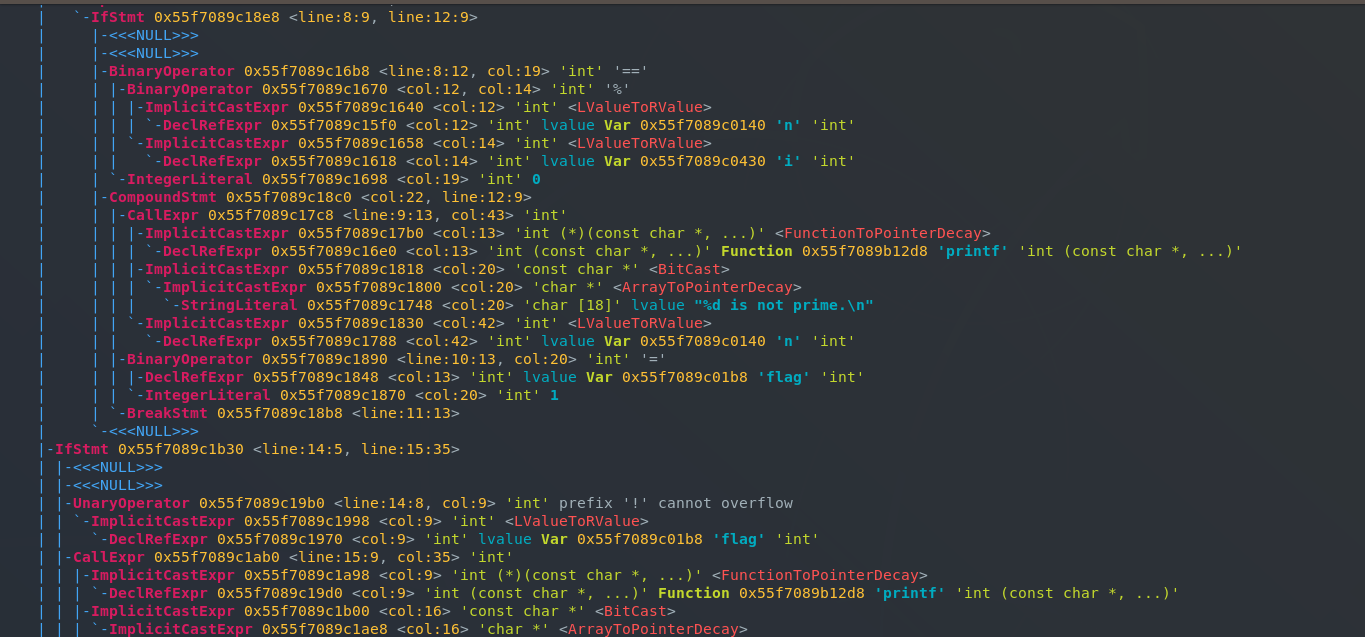
\includegraphics[scale=0.3]{AST.png}
\caption{Sample AST}
\label{fig:AST Example}
\end{figure}

These major statements occurred in the AST's.

\subsubsection{if-stmt}
It consists of a conditional Expr(BinaryOperator) and two Stmts, one for the then-case and one for the else-case respectively.

\subsubsection{CompoundStmt}
Compound statements are made up of two or more program statements that are executed together.

\subsubsection{DeclStmt}
This is used for declaration and initialization of variables.\\
It consists of:\\
\\
\textbf{1. Declaration part:}
\begin{minted}{css}
VarDecl 0x55f7089c0140 <col:5, col:9> col:9 used n 'int'
\end{minted}
\textbf{2. Initialization part:}
\begin{minted}{css}
IntegerLiteral 0x55f7089c0218  <col:19> 'int' 0
\end{minted}

\subsubsection{FucntionDecl}
This denotes the function along with its parameters and return type.

\subsubsection{for-stmt}
This consists of declaration step, condition step, and increment step.\\
If consists of: \\
\\
\textbf{1. This declares an \textit{int i}.}
\begin{minted}{css}
DeclStmt 0x55f7089c04b0 <line:7:9, col:16>
\end{minted}
\\
\textbf{2. This acts as an condtional statement.}
\begin{minted}{css}
BinaryOperator 0x55f7089c1580  <col:18, col:20>  'int' '<'
\end{minted}
\\
\textbf{3. This is the increment step.}
\begin{minted}{css}
UnaryOperator 0x55f7089c15d0 <col:23, col:24>'int' postfix '++'
\end{minted}

\subsubsection{printf-stmt}
Using ImplicitCastExpr() for casting string to a constant char* from a char array as a pointer with DeclRefExpr() referencing to \textbf{printf}.
\begin{minted}{css}
ImplicitCastExpr 0x55f7089c17b0 <col:13>'int (*)(const char *, ...)'
<FunctionToPointerDecay>
\end{minted}

\section{AST Traversals}
\textbf{Visitor Pattern :} It is a technique (Object Oriented pattern) to separate data structure definitions from code that traverses the structure of AST.

\subsection{Create a FrontendAction}
FrontendAction is an interface that allows execution of user specific actions as part of the compilation. 

\subsection{Create a ASTConsumer}
ASTConsumer is an interface used to write generic actions on an AST, regardless of how the AST was produced.

\subsection{Use the RecursiveASTVisitor}
The Recursive AST Visitor enables you to traverse the nodes of Clang AST in a depth-first manner. We visit specific nodes by extending the class and implementing the desired \textit{Visit*} method

\subsection{Accessing the SourceManager and ASTContext}
Information like source locations and global identifier information, are not stored in the AST nodes themselves, but in the ASTContext and its associated source manager. To retrieve them we need to hand the ASTContext into our RecursiveASTVisitor implementation.

\section{Error messages}
The \textbf{assert} mechanism is used to check the preconditions and assumptions, which might be caught early, hence reducing the debugging time significantly.\\
\\
If the first argument of the assert turns out to be false, it will terminate the program(preferably giving a message).\\
Example:
\begin{minted}{c}
inline Value *getOperand(unsigned I) {
  assert(I < Operands.size() && "getOperand() out of range!");
  return Operands[I];
}
\end{minted}
\\
In this example, if the argument size is greater than \textbf{Operands.size()}, the program is terminated and an error message is printed "\textit{getOperand() out of range!}".\\
\\
\textbf{Assertions} can also be made to indicate a peice of code that should not be reached. With \textbf{assertions enabled}, the following will print the message if ever reached, and exits:
\begin{minted}{c}
llvm_unreachable("Code should not be reached here.");
\end{minted}
\\
But we should remember that it both assert and llvm\_unreachable wont exit the program in the release mode.

\section{LLVM-IR}
LLVM front end converts the OpenCL program into \textbf{LLVM IR}, an intermediate presentation that is intended to be used as input for the LLVM compiler back end. The back end is then responsible for translating the LLVM IR into target specific language which is usable by the parallel computing capable hardware, for example GPU.\\
\\
To get the LLVM-IR, the following command is run:
\begin{minted}{c}
./clang -S -emit-llvm test.cpp -o test.ll
\end{minted}
\\
This is what an \textit{.ll} file looks like:
\begin{minted}{css}
; ModuleID = 'test.cpp'
source_filename = "test.cpp"
target datalayout = "e-m:e-i64:64-f80:128-n8:16:32:64-S128"
target triple = "x86_64-unknown-linux-gnu"

; Function Attrs: noinline nounwind optnone uwtable
define dso_local void @_Z3sumii(i32 %a, i32 %b) #0 {
entry:
  %a.addr = alloca i32, align 4
  %b.addr = alloca i32, align 4
  %c = alloca i32, align 4
  store i32 %a, i32* %a.addr, align 4
  store i32 %b, i32* %b.addr, align 4
  %0 = load i32, i32* %a.addr, align 4
  %1 = load i32, i32* %b.addr, align 4
  %add = add nsw i32 %0, %1
  store i32 %add, i32* %c, align 4
  ret void
}

; Function Attrs: noinline norecurse nounwind optnone uwtable
define dso_local i32 @main() #1 {
entry:
  %retval = alloca i32, align 4
  store i32 0, i32* %retval, align 4
  call void @_Z3sumii(i32 1, i32 2)
  ret i32 0
}

\end{minted}
\\
Some main highlights of LLVM IR are:
\subsection{Comments}
Comments in LLVM assembly begin with a semicolon (;) and continue to the end of the line.

\subsection{Declaration of Function}
To declare a function, begin the declaration with the declare keyword followed by the return type, the function name, and an optional list of arguments to the function.\\
The declaration must be in the global scope. Eg. \begin{minted}{css}
 declare i32 puts(i8*)
\end{minted}

\subsection{Defining a Function}
To define a function, begin with the define keyword followed by the return type, and then the function name. Eg.\begin{minted}{css}
 define i32 @main()
\end{minted} 

\subsection{Calling a Function}
To call the function, call \textbf{\textless function return type\textgreater \textless function name\textgreater \textless optional function arguments\textgreater}

\subsection{Returning a Function}
Each function ends with a return statement. There are two forms of return statement: \textbf{ret \textless type\textgreater \textless value\textgreater} or \textbf{ret void}.

\subsection{Declaring a vector/array}
You declare a vector or array type as \textbf{[no. of elements X size of each element]}.

\subsection{Global identifiers}
Global identifiers begin with the at (@) character. All function names and global variables must begin with \textbf{@}, as well.

\subsection{Local identifiers}
Local identifiers in the LLVM begin with a percent symbol (\%). The typical regular expression for identifiers is \textbf{[\%@][a.zA.Z\$.\_][a.zA.Z\$.\_0.9]*}.

\subsection{Declaring global string}
You declare a global string constant for the myname string as follows: \textbf{@myname = constant [13x i8] c"Hello World!\textbackslash00"}\\
Example from code:\\
\begin{minted}{css}
@.str = private unnamed_addr constant [3 x i8] c"%d", align 1
\end{minted}

\subsection{For conditionals}
It is divided into 3 parts: \\
\textbf{for.cond:} - The conditional statement of \textit{for}.\\
\textbf{for.body:} - The body of the \textit{for} statement.\\
\textbf{for.inc:} - The increment condition of \textit{for} statement.

\section{Assembly language}
Consider a simple cpp program:

\begin{minted}{cpp}
void sum(int a, int b, int c) {
    int d = a + b + c;
}
void sum(int a, int b) {
    int c = a + b;
}
int main() {
    sum(1, 2, 3);
    sum(1, 2);
    return 0;
}
\end{minted}
\\
To get the assembly code, the following command is run:
\begin{minted}{c}
./clang -S test.cpp -o test.s
\end{minted}
\\
The assembly code generated for a cpp program with function overloading is: 

\begin{minted}{css}
	.file	"test.cpp"
	.text
	.globl	_Z3sumiii
	.type	_Z3sumiii, @function
_Z3sumiii:
.LFB0:
	.cfi_startproc
	pushq	%rbp
	.cfi_def_cfa_offset 16
	.cfi_offset 6, -16
	movq	%rsp, %rbp
	.cfi_def_cfa_register 6
	movl	%edi, -20(%rbp)
	movl	%esi, -24(%rbp)
	movl	%edx, -28(%rbp)
	movl	-20(%rbp), %edx
	movl	-24(%rbp), %eax
	addl	%eax, %edx
	movl	-28(%rbp), %eax
	addl	%edx, %eax
	movl	%eax, -4(%rbp)
	nop
	popq	%rbp
	.cfi_def_cfa 7, 8
	ret
	.cfi_endproc
.LFE0:
	.size	_Z3sumiii, .-_Z3sumiii
	.globl	_Z3sumii
	.type	_Z3sumii, @function
_Z3sumii:
.LFB1:
	.cfi_startproc
	pushq	%rbp
	.cfi_def_cfa_offset 16
	.cfi_offset 6, -16
	movq	%rsp, %rbp
	.cfi_def_cfa_register 6
	movl	%edi, -20(%rbp)
	movl	%esi, -24(%rbp)
	movl	-20(%rbp), %edx
	movl	-24(%rbp), %eax
	addl	%edx, %eax
	movl	%eax, -4(%rbp)
	nop
	popq	%rbp
	.cfi_def_cfa 7, 8
	ret
	.cfi_endproc
.LFE1:
	.size	_Z3sumii, .-_Z3sumii
	.globl	main
	.type	main, @function
main:
.LFB2:
	.cfi_startproc
	pushq	%rbp
	.cfi_def_cfa_offset 16
	.cfi_offset 6, -16
	movq	%rsp, %rbp
	.cfi_def_cfa_register 6
	movl	$3, %edx
	movl	$2, %esi
	movl	$1, %edi
	call	_Z3sumiii
	movl	$2, %esi
	movl	$1, %edi
	call	_Z3sumii
	movl	$0, %eax
	popq	%rbp
	.cfi_def_cfa 7, 8
	ret
	.cfi_endproc
.LFE2:
	.size	main, .-main
	.ident	"GCC: (Ubuntu 7.3.0-16ubuntu3) 7.3.0"
	.section	.note.GNU-stack,"",@progbits

\end{minted}
\\
C++ supports function overloading, i.e., there can be more than one functions with same name and differences in parameters.\\
This technique of adding additional information to function names is called \textbf{Name Mangling}. C++ standard doesn’t specify any particular technique for name mangling, so different compilers may append different information to function names. \\
\\
The two functions sum are referenced by same name, but differs in the number of parameters(One has 2 and another has 3 parameters).\\
\\
\textbf{clang} adds a \textbf{Z} followed by length of function name in int followed by the function name and then followed by argument type’s abbreviation.\\
\\
In the example the compiler differentiates them by referring them as: \\
\textbf{\_Z3sumiii} - Here the 3 i's show that the number of parameters are 3.\\
\textbf{\_Z3sumii} - Here there are 2 i's, which show that number of parameters are 2.\\

\section{Compiler toolchain and options}
\subsection{Compiler Frontend - clang}\\
\textbf{-emit-ast} : Generate the clang AST files.\\
\textbf{-emit-llvm} : Use llvm representation for assembler and object files.\\
\textbf{-c} : Only run preprocess, compile, and assemble steps.\\
\textbf{-E} : Only run the preprocessor.\\

\subsection{Compiler Middle end}
\textbf{llvm-as} : Converts a LLVM assembly file into LLVM bitcode.\\
\textbf{llvm-dis} : Converts LLVM bitcode to LLVM assembly language.

\subsection{Optimizer}
\textbf{-dot-callgraph} : It prints the call graph.\\
\textbf{-dot-cfg} : This prints the cfg graph.\\
\textbf{-O1, -O2, -O3} : These options are for optimization levels, in increasing order of aggressiveness.\\
\textbf{-Osize} : This optimizes the binary for file size.\\
\textbf{--ffast-math} : This enables lossy optimization for floating point operations.

\section{Kaleidoscope}
\textbf{Kaleidoscope} is a procedural language that allows you to use conditionals, define functions, math, etc.\\
The only data type in Kaleidoscope is a 64-bit floating point type. Hence, the language doesn't require type declarations.\\
Example code:
\begin{minted}{python}
# Compute the x'th fibonacci number.
def fib(x)
  if x < 3 then
    1
  else
    fib(x-1)+fib(x-2)

# This expression will compute the 40th number.
fib(40)
\end{minted}
\\
The external library functions are used by using the '\textbf{extern}' keyword before the funciton name.

\subsection{Lexer for Kaleidoscope}
The \textbf{Lexer} breaks the input into "\textit{tokens}". Each token contains some metadata and a token code.\\
This is what it looks like:

\begin{minted}{c}
// The lexer returns tokens [0-255] if it is an unknown character, otherwise one
// of these for known things.
enum Token {
  tok_eof = -1,

  // commands
  tok_def = -2,
  tok_extern = -3,

  // primary
  tok_identifier = -4,
  tok_number = -5,
};

static std::string IdentifierStr; // Filled in if tok_identifier
static double NumVal;             // Filled in if tok_number
\end{minted}
\\
The implementation of lexer function is done using a single function \textit{gettok()}. The definition is as follows:
\begin{minted}{c}
// gettok - Return the next token from standard input.
static int gettok() {
  static int LastChar = ' ';

  // Skip any whitespace.
  while (isspace(LastChar))
    LastChar = getchar();
\end{minted}
\\
The \textbf{gettok} function is called to return the next token from standard input.

\bibliographystyle{plain}
\bibliography{references}
\textbf{http://llvm.org/docs/GettingStarted.html#check-here}\\
\textbf{http://clang.llvm.org/docs/IntroductionToTheClangAST.html}\\
\textbf{https://llvm.org/docs/CodingStandards.html#assert-liberally}\\
\textbf{http://llvm.org/docs/tutorial/LangImpl01.html}\\
\textbf{https://en.wikipedia.org/wiki/Name\_mangling}\\
\textbf{https://gist.github.com/zchee/48be861fcc3c5239ec1954b34d9a5205}\\
\textbf{https://gist.github.com/zchee/48be861fcc3c5239ec1954b34d9a5205}

\end{document}
